\documentclass[12pt, oneside]{scrbook}   	% use "amsart" instead of "article" for AMSLaTeX format
\usepackage{geometry}                		% See geometry.pdf to learn the layout options. There are lots.
\geometry{letterpaper}                   		% ... or a4paper or a5paper or ... 
%\geometry{landscape}                		% Activate for for rotated page geometry
%\usepackage[parfill]{parskip}    		% Activate to begin paragraphs with an empty line rather than an indent
\usepackage{graphicx}				% Use pdf, png, jpg, or eps"§ with pdflatex; use eps in DVI mode
								% TeX will automatically convert eps --> pdf in pdflatex		
\usepackage{fontspec}
\usepackage{amssymb}
\usepackage{listings}
\usepackage{hyperref}
\hypersetup{colorlinks=true, linkcolor=red}
\usepackage[most]{tcolorbox}
%\usepackage{minipage}

\setmainfont{Times New Roman}

\usepackage{fancyhdr}
\pagestyle{fancy}

\fancyhf{}
\fancyhead[R]{\rightmark}
\fancyfoot[R]{\thepage}

\title{LMEDS 2.4 Instruction Manual}
\titlehead{\centering
\includegraphics{lmedslogo}}
\author{Tim Mahrt}
\date{November 2, 2016}

\renewcommand\thesection{\arabic{section}}

\setcounter{secnumdepth}{3}

\begin{document}

\maketitle

\newpage

\paragraph{}

It is my hope that you will find this document useful in working with LMEDS. This document contains information for all aspects of LMEDS, from installation and setup, to creating experiments, running experiments, and obtaining and analyzing test results.  If you have any questions, comments, or other feedback, please contact me at timmahrt@gmail.com

\vspace{25mm}

Special thanks goes to those who used early versions of LMEDS and provided critical feedback, feature requests, and bug reports (in alphabetical order):

\vspace{5mm}

Stefan Baumann

Jennifer Cole

Núria Esteve Gibert

Martine Grice

Jonathan Howell

José I. Hualde

Suyeon Im

Preethi Jyothi

Janina Kalbertodt

Amelia Kimball

Caroline Smith

\vspace{5mm}

and the more than 1000 people on Mechanical Turk who have participated in experiments using LMEDS!

\vfill

\begin{tcolorbox}[breakable,colback=white,colframe=green,width=\dimexpr\textwidth+12mm\relax,enlarge left by=-6mm]

\textbf{Development of LMEDS was possible thanks to }
\begin{itemize}
\item NSF grant BCS 12-51343 to
Jennifer Cole, José I. Hualde, and Caroline Smith
\item A*MIDEX project
(n° ANR-11-IDEX-0001-02) to James Sneed German funded by the
Investissements d'Avenir French Government program,
managed by the French National Research Agency (ANR).
\end{itemize}

\end{tcolorbox}

\tableofcontents

\newpage

% !TEX root = LMEDS_manual.tex

%%%%%%%%%%%%%%%%%%%%%
\section{Orientation}
%%%%%%%%%%%%%%%%%%%%%

LMEDS comes packaged with the following folders:

\begin{itemize}
\item cgi-bin

Small code snippets (with the extension .cgi) go here--one for each experiment

\item html

Contains static HTML, Javascript, and CSS files

\item imgs

Image files used by LMEDS

\item lmeds

The main repository for code.

\item lmeds/user\_scripts

Within the lmeds code directory are some scripts that users can use in setting up their experiments and in post-processing their data.

\item tests

Holds the resource files for each experiment

\item user\_manual

Contains the user manual

\end{itemize}

\paragraph{}

If you are creating an experiment, you'll need to add one file to cgi-bin and you'll need to add a folder to tests, containing all of the resource files used in the experiment--the other folders can all be ignored. The next section goes into the details of how to create the 

\subsection{Getting started with LMEDS}

This manual describes how to create files used by LMEDS from scratch.  You might find it useful to reference the experiment files that come with LMEDS, located in /tests/lmeds\_demo.  In it, you'll find an example dictionary (english.txt), sequence file (sequence.txt), input files contained in the (audio/ and txt/ folders), survey files (presurvey.txt and postsurvey.txt), and some sample output files (stored in the folder output/).
\textbf{When you are starting a new experiment from scratch, you might find it useful to start with the demo files provided.}

\begin{figure}
\subsection{LMEDS Workflow Schematic}
\centering
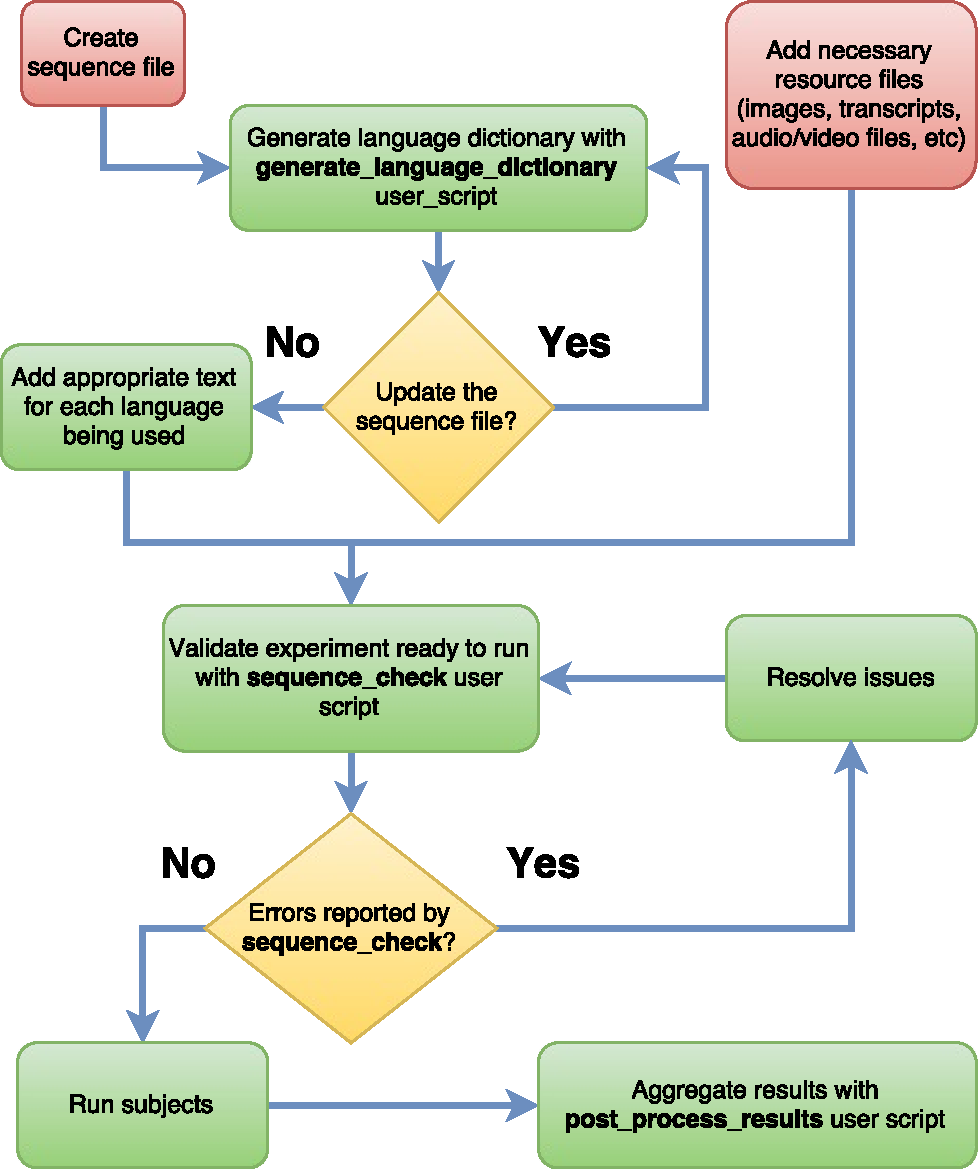
\includegraphics[height=0.95\textheight]{lmedsSchematic.pdf}
\end{figure}


\paragraph{}

To begin an LMEDS experiment, two things are needed--resource files and a sequence file (the two boxes in red).  Once the sequence file is sufficient for your purposes, a language dictionary is generated from it with the user script generate\_language\_dictionary.  If any changes are made to the sequence file, the language dictionary will need to be regenerated.  Once the sequence file and language dictionary are syncronized, enter the appropriate text for each language being used.

\paragraph{}
With the sequence files, resource files, and generated language dictionary, validate that the experiment can be run using sequence\_check.  sequence\_check will ensure that all resources and text specified in the sequence file are available and that each page in the sequence file can be created.  As long as there are issues, resolve them and run the script again.  Once there are no reported errors, test it for yourself and then run subjects.  After collecting all subject data, use post\_process\_results to aggregate the user data.




% !TEX root = LMEDS_manual.tex

%%%%%%%%%%%%%%%%%%%%%
\section{Notices and warnings}
%%%%%%%%%%%%%%%%%%%%%

\subsection{Creating and editing text files}

\paragraph{}

The input and outputs to LMEDS shouldn't be edited in a word processor.  A plain text editor should be used.  The text editors that come with most operating systems (notepad on Windows or Text Edit on mac) should be suitable however, you may want a more developed plain text editor.  I have personal experience with NotePad++, Gedit, and TextWrangler, which are all freely available tools.  If you search online, you can find reviews for editors that might suit you better.

\subsection{No spaces in names}

\paragraph{}

Please do not include spaces in folder or file names.  If you have a file composed of multiple words, either do not use spaces or use underscores.  E.g. for a folder that you want to call ``lmeds demo'', reasonable names include ``lmeds\_demo'' or ``lmedsDemo'' or ``lmedsdemo''.

\subsection{Errors in LMEDS}

\paragraph{}

LMEDS was written in python.  If something goes wrong (an unexpected or anticipated error) python will print out a formatted error report called a \textbf{stack trace}.  Unintuitively, the direct cause of the error is printed at the \textbf{bottom} of this report.  

\paragraph{}
While the stack trace can be difficult to understand for non-programmers, usually the direct cause is printed as reasonably understandable English.  For example the last line in the stack trace might be \textit{ERROR: Folder, ../tests/lmeds\_demo, does not exist} or it might be \textit{Text key axb\_instructions not in dictionary file english.txt.  Please add text key to dictionary and try again.'}

\paragraph{}
Errors are common when designing a new experiment (although the included script /lmeds/user\_scripts/sequence\_check.py can be used to automatically find common errors like missing resource files or incorrectly specified page definitions).  If an error occurs, don't panic.  Consult the error log as specified above.  If you are unsure about the error, please send it to me.

\end{tcolorbox}



% !TEX root = LMEDS_manual.tex

%%%%%%%%%%%%%%%%%%%%%
\section{Creating your own experiments}
%%%%%%%%%%%%%%%%%%%%%

%%%%%%%%%%%%%%%%%%%%%
\subsection{User-defined test components}
%%%%%%%%%%%%%%%%%%%%%

An LMEDS test has the following components


%%%%%%%%%%%%%%%%
\subsubsection{Audio and video files}

\paragraph{}
An audio file can be any common type (.mp3, .wav, etc.) and a video file can be one of (.mp4, .ogg, or .webm).   Some web browsers are unable to play audio in certain file types.  Personally, I encode every audio file as both .mp3 and .ogg and every video file as .mp4 and .ogg.  I recommend encoding each file in two different formats.  If a user is unable to load one file format, their browser will automatically load the other file format.

\paragraph{}
See the following pages for more information on browser compatibility:

\url{http://www.w3schools.com/tags/tag\_audio.asp}

\url{http://www.w3schools.com/html/html5_video.asp}

\paragraph{}
For audio files, audacity makes it very easy to convert entire directories of audio files into multiple audio formats with it's `chain' functionality.  

\url{http://audacityteam.org/}

\paragraph{}
To save server space and speed up loading times for users with slower internet, I reencode my wav files to 16,000 HZ before I convert them to .mp3 and .ogg.  This step is not required.  Sox is a freely available command line tool that can do this task easily:

\begin{lstlisting}
sox input_file_name -r 16000 output_file_name rate -v 96k
\end{lstlisting}

\url{http://sox.sourceforge.net/}


%%%%%%%%%%%%%%%%
\subsubsection{Transcription files}

\paragraph{}
Only raw txt files with the extension .txt are accepted.  Each transcription file should contain the transcript for one stimulus.

\paragraph{}
For long excerpts, you should specify the line breaks explicitly by chunking the text into pieces over the span of several lines.  For a long excerpt, if all of the text lies on one line, the text will run off the page in LMEDS.


%%%%%%%%%%%%%%%%
\subsubsection{Sequence file (see section \ref{sec:sequenceSpec})}

\paragraph{}
The file that specifies the control flow of a test.  It specifies what instructions and stimuli users will be presented with in a test and in what order. 

\paragraph{}
Multiple sequence files can exist for a set of audio and transcription files (e.g. one could have a sequence with the stimuli in a certain order and another sequence with the stimuli in a different order or with different instructions, etc.).


%%%%%%%%%%%%%%%%
\subsubsection{Dictionary file(s) (see section \ref{sec:dictionarySpec})}

\paragraph{}
The file that contains all text that will be seen by users in your experiment.  This file is independent of a sequence file so one could write a sequence and present it in both English and Russian, for example.


%%%%%%%%%%%%%%%%
\subsubsection{Survey file(s) (see section \ref{sec:surveySpec})}

\paragraph{}
A survey file can be used to get various kinds of feedback, such as might be needed for a longform survey or a short-answer question.  Supports text boxes, checkboxes, and radio buttons.

\paragraph{}
Each survey requires its own survey file (e.g. presurvey.txt, postsurvey.txt).

\paragraph{}
Most pages have a static layout (defined in the python code) that is filled in with the same type of content.  A survey is different because the amount of content and inputs vary with each survey page, whereas all AXB pages, for example, share the same number of inputs and outputs.  For this reason, each survey requires its own specification file while other types of pages do not.


%%%%%%%%%%%%%%%%
\subsubsection{.CGI file}

\paragraph{}
The file that defines a single experiment--via a sequence file and a language file.  The name given to this file (e.g. lmeds\_demo.cgi) is the name that participants would use to access the experiment in the URL.

\paragraph{}
A template of a typical .cgi file can be found in section \ref{sec:cgitemplate}.  An example file is also distributed in the /cgi folder included with LMEDS.


%%%%%%%%%%%%%%%%%%%%%
\subsection{Dictionary file specification}
\label{sec:dictionarySpec}
%%%%%%%%%%%%%%%%%%%%%

\paragraph{}
LMEDS uses \textbf{dictionaries} for multi-lingual support.  These dictionaries contain a set of keys where each key has text associated with it.  One dictionary might have text only in English, while another only in French, but the keys are the same in both.  Thus, when a key is used in a page, LMEDS looks in the dictionary (that is appropriate for the current experiment) for the corresponding text for that key.  E.g. the key ``dictionary'' will fetch the text ``Dictionary'' for English and  ``Dictionnaire'' for French.  Each dictionary file is created by the user.

\paragraph{}
Some keys are defined within the python code.  Other keys are user-defined.  The user\_script \textbf{generate\_language\_dictionary.py} can be used to generate a template dictionary file (all keys are present but there are no text values) or update an existing dictionary file with new keys.

\paragraph{}
You might find it useful to create a new dictionary by using another one--either if you're starting a new experiment or translating your current experiment into another language.

\paragraph{}
A dictionary files has the following components (a very small, but complete dictionary file follows these, alternatively, you can look at the included dictionary file for a real example: \textbf{/tests/lmeds\_demo/english.txt}):


%%%%%%%%%%%%%%%%
\subsubsection{Sections}

\paragraph{}
A section is denoted with ``-'' characters on the line above and below the section name.  The lengths of these lines (the number of ``-'') doesn't matter but should be kept the same length to be visually more coherent.  

\paragraph{}
Sections are actually ignored in the code.  Their only purpose is to help structure dictionaries, perhaps most naturally by page type.  Keys shared by multiple pages are kept in their own sections.


%%%%%%%%%%%%%%%%
\subsubsection{Keys}

\paragraph{}
A key is denoted in the same way with ``='' characters.  Keys must be the same, regardless of the language. 


%%%%%%%%%%%%%%%%
\subsubsection{Texts}

\paragraph{}
A ``text'' appears after a key and before another key or section.  Unlike sections and keys, text is undecorated text.  

\paragraph{}
Text is rendered in HTML.  This means HTML markup is allowed.  It also means that whitespace other than a single space is ignored, although you may use extra whitespace to make it easier to read the text in the dictionary.  If you want a line break, for example, you will need to insert one used \texttt{<br />}


%%%%%%%%%%%%%%%%
\subsubsection{Dictionary example file}

\paragraph{}
Here is a short, concrete example of a dictionary file

\paragraph{}

\begin{tcolorbox}[colback=white,colframe=blue,width=\dimexpr\textwidth+12mm\relax,enlarge left by=-6mm]

\begin{lstlisting}
---------------
text_page
---------------

===============
title
===============

Perception of Spoken Discourse

===============
first_block_finished
===============

You have completed the first block.<br /><br />

Please feel free to rest for a minute before continuing.

\end{lstlisting}

\end{tcolorbox}

\paragraph{}
The section denotes that these keys are used in the text pages, which tend to be used for giving instructions.  Whenever LMEDS needs to display the title, it will look at the text for the key ``title'' in this case ``Perception of Spoken Discourse''.


%%%%%%%%%%%%%%%%%%%%%
\subsection{Survey file specification}
\label{sec:surveySpec}
%%%%%%%%%%%%%%%%%%%%%

\paragraph{}
The survey format allows for the simple creation of short or long questionnaires.  The format is simple--the first line in a survey question contains the text prompt, subsequent lines specify one or more data entry fields that users can use to answer the question, and, finally, a blank line signals that the current item is complete. An small example survey file can be found is at the bottom of this section, two surveys are also bundled in lmeds \textbf{/tests/lmeds\_demo/presurvey.txt} and \textbf{/tests/lmeds\_demo/postsurvey.txt}.

\paragraph{}
A note on arguments: For data entry fields that have arguments, arguments should be separated from the data entry field name by a space and from each other by a comma 

e.g.

\begin{lstlisting}
Choice English, Arabic, Other
\end{lstlisting}

\paragraph{}
Here is the list of data entry fields available:


%%%%%%%%%%%%%%%%
\subsubsection{None}

\paragraph{}
There are no inputs the user can choose from.  This is used to include instructions on the page.

e.g.

\begin{lstlisting}
Please answer the questions below.
None
\end{lstlisting}


%%%%%%%%%%%%%%%%
\subsubsection{Choice}

\paragraph{}
Users can select exactly one item out of many.

e.g.

\begin{lstlisting}
Sex:
Choice Male, Female
\end{lstlisting}


%%%%%%%%%%%%%%%%
\subsubsection{Item\_List}

\paragraph{}
Users can select as many items as they want out of many.

e.g.

\begin{lstlisting}
Indicate the language(s) that you are familiar with.
Item_List English, French, Spanish, Italian, German
\end{lstlisting}


%%%%%%%%%%%%%%%%
\subsubsection{Choicebox}

\paragraph{}
A dropdown box.  Users can select one item from many.  Similar to a \textbf{Choice} but is more efficient in space for large lists of items.

e.g.

\begin{lstlisting}
Level of education completed:
Choicebox High School, Some College, Bachelor's Degree
\end{lstlisting}


%%%%%%%%%%%%%%%%
\subsubsection{Sliding\_Scale}

\paragraph{}
A sliding scale.  Specify the numerical scale (which controls the granularity of the user's choice) and the labels for the two extremes of the scales.

e.g.

\begin{lstlisting}
How satisfied were you with this experiment?
Sliding_Scale 0, 100, Very Unsatisfied, Very Satisfied
\end{lstlisting}


%%%%%%%%%%%%%%%%
\subsubsection{Textbox}

\paragraph{}
A single line for users to enter a small amount of information.  A textbox takes no arguments.

e.g.

\begin{lstlisting}
Occupation
Textbox
\end{lstlisting}


%%%%%%%%%%%%%%%%
\subsubsection{Multiline\_Textbox}

\paragraph{}
A longer-form textbox that can span several lines.  It takes exactly two arguments: the number of characters across and the number of lines.

e.g.

\begin{lstlisting}
What did you think of this test?  Please provide any feedback.
Multiline_Textbox 50, 7
\end{lstlisting}


%%%%%%%%%%%%%%%%
\subsubsection{Sublists}

\paragraph{}
It is possible to designate a group of items as subquestions of the previous question.  These items will be displayed tabbed.  To do this, encapsulate the relevant items in the sublist tag:

\begin{lstlisting}
<sublist>
Occupation
Textbox

City of birth
Textbox
</sublist>
\end{lstlisting}


%%%%%%%%%%%%%%%%
\subsubsection{Survey file example}

\paragraph{}
Here is a short concrete example demonstrating the key features discussed above

\paragraph{}

\begin{tcolorbox}[colback=white,colframe=blue,width=\dimexpr\textwidth+12mm\relax,enlarge left by=-6mm,enlarge right by=6mm]

\begin{lstlisting}
Please answer the questions below.
None

Sex: 
Choice Male, Female

Age:
Textbox

Country of birth:
Choice United States, Other
Textbox

<sublist>
If United States, list city/state:
Textbox

If other, how old were you when you moved to the USA?
Textbox
</sublist>

\end{lstlisting}

\end{tcolorbox}

\paragraph{}
Thus we have a survey with (ignoring the first item, which doesn't take user input) 5 items in total (2 being subitems).  The third item shows how multiple data entry fields can be placed on a single question (if the user selects ``other'' for the first question they are expected to specify what they meant in the Textbox).


%%%%%%%%%%%%%%%%%%%%%
\subsection{Sequence file specification}
\label{sec:sequenceSpec}
%%%%%%%%%%%%%%%%%%%%%

\paragraph{}
The sequence file contains the items that will be presented in a test.  The first line in a test is the test name which should be prefixed with a ``*'' (e.g. *My\_Test\_Sequence) (\textbf{data from the experiment will be output to a folder with the test name.  Giving multiple sequence files the same name, means that they will dump their output to the same folder}).  The second item must be ``login'' where users create a name to associate their data with.  If login is not the item on the second line, unexpected behavior can result.
Subsequent items are presented in a linear fashion as users progress through the sequence.  The last item in the sequence must be ``end''.

\paragraph{}
\textbf{Most pages take arguments.}  These arguments specify the behavior the page should take (which audio files to play, instructions to present, etc.)  Arguments are separated from one another and from the page type by a space.  Audio files and textfiles included in an argument should not include their file extension (.txt, .wav, etc.)--LMEDS will determine the appropriate extension to be used.

\begin{lstlisting}
Prominence water water 1 3 true
\end{lstlisting}

\paragraph{}
The above example is the entry for the prominence page.  It comes with 5 arguments.  Sections \ref{sec:sequenceSpecBasic} and \ref{sec:sequenceSpecSpecific} include information on how to understand the individual arguments to a page.  A full example sequence file can be found in section \ref{sec:sequenceFileExample}.


%%%%%%%%%%%%%%%%
\subsubsection{A Note on Default Values}

\paragraph{}
\textit{This is a completely optional feature.  If you find it confusing you can skip it.}

\paragraph{}
Some page types, such as \textbf{prominence} have default values for some arguments.   An argument might have a default value if alternative values are uncommon or to support new functionality without requiring changes to pre-existing code.

\paragraph{}
Arguments that have default values do not have to be specified in a sequence file if you are ok with the defaults--this can make your sequence file cleaner and easier to read and maintain.

\paragraph{}
There are two ways that you can specify an optional value.  One is to list it as normal e.g.

\begin{lstlisting}
prominence water water 1 3 p_ac_instr true
\end{lstlisting}

\paragraph{}
A second way is to refer to it explicitly by its name as described in sections \ref{sec:sequenceSpecBasic} and \ref{sec:sequenceSpecSpecific}. e.g.

\begin{lstlisting}
prominence water 1 3 instructions=p_ac_instr presentAudio=true
\end{lstlisting}

\paragraph{}
This second way is useful, for example, if you wanted to specify the value for a later variable such as ``presentAudio'' but not ``instructions''.  The only way to do this is by naming the variable 

\begin{lstlisting}
Prominence water 1 3 presentAudio=true
\end{lstlisting}

\paragraph{}
If one attempted the same list of arguments but without referring to the variable name, this would set ``instructions=true'' which would cause an error unless instructions named ``true'' existed in the dictionary file.

\begin{lstlisting}
Prominence water 1 3 true
\end{lstlisting}


\subsubsection{Valid Keyboard Keys}
\label{sec:validKeys}


\paragraph{}
Some pages allow interaction with the keyboard (such pages will direct you to this section).  For those pages, experimenters can specify any letter or number on their keyboard, like so

\begin{lstlisting}
somePage playAudioKey=p
\end{lstlisting}

\paragraph{}
If we suppose that `playAudioKey' specifies the button that plays an audio recording, pressing the `p' button on the keyboard would play audio.

\paragraph{}
What about something like the `enter' key?  The following codes can be entered to have their associated button registered as the key:  \textbf{alt, backspace, capslock, ctrl, enter, escape, shift, space, and tab}.  And they can be used like

\begin{lstlisting}
somePage playAudioKey=enter
\end{lstlisting}


%%%%%%%%%%%%%%%%
\subsubsection{Sequence file example}
\label{sec:sequenceFileExample}

\paragraph{}
Unlike the below example, in a sequence file each page description should fit on one line.  In this example, for the purposes of space, some pages span several lines.  A proper example sequence file is also distributed with the lmeds source:

\textbf{/LMEDS/tests/lmeds\_demo/sequence.txt}

\paragraph{}

\begin{tcolorbox}[colback=white,colframe=blue,width=\dimexpr\textwidth+12mm\relax,enlarge left by=-6mm,enlarge right by=6mm]

\begin{lstlisting}
*LMEDS_Demo
login

text_page demo_instructions
consent demo_consent
survey presurvey

media_list audio 1 1 1 [water apples water]
media_choice same_different_instr audio 0.5 1 -1
	[[water apples]] [same different]
boundary_and_prominence water water 0 -1
	boundary_instr prominence_instr true
boboundary_and_prominence apples apples 2 2 
	boundary_instr prominence_instr true
end
\end{lstlisting}
\end{tcolorbox}


%%%%%%%%%%%%%%%%%%%%%
\subsection{Sequence file specification - randomizing stimulus order}
\label{sec:sequenceSpecRandom}
%%%%%%%%%%%%%%%%%%%%%

\paragraph{}
A short but important section.  The sequence file presents the order that all participants will encounter the stimuli.  For many experiments however, it is necessary that the stimuli be presented in a different order for each experiment participant--to account for affects of stimulus order for example. 

\paragraph{}
\textbf{Technical details} Here is a brief explanation of how randomization is performed by LMEDS.  LMEDS presents materials based on the order presented in a sequence file.  In order to present each user with the stimuli presented in a random order, each user must get their own sequence file.  When instructed to do randomization, LMEDS reads in the sequence file created by the experimenter, randomizes the order of the stimuli, and then creates a new sequence file.  It then reloads that file and begins the experiment.

\paragraph{}
The following instructions show how sequence randomization can be implemented in a sequence file.

\begin{enumerate}
\item Indiciate to LMEDS that you want to randomize a sequence:

In the .cgi file, in the function 'runExperiment' include the line \textbf{individualSequences=True}

\item Specify which portions should be randomized

In the sequence file, surround the section to be randomized with the following two lines\\
	\textbf{<randomize>} \\
	\textbf{</randomize>}

\item Create a folder where the user-specific sequence files will be placed by LMEDS.
/LMEDS/tests/<test root folder name>/individual\_sequences/<first line in sequence file>/
\end{enumerate}

\paragraph{}
So, for a short concrete example, here is how the above three would look in practice


\begin{lstlisting}
experiment_runner.runExperiment(`lmeds_demo',
                                `sequence_randomized.txt',
                                `english.txt',
                                individualSequences=True)
\end{lstlisting}

\paragraph{}
and 

\begin{lstlisting}
*LMEDS_Simple_Randomized_Demo
login
text_page same_different_randomized_instructions
<randomize>
media_choice choice_instr audio 0.0 -1 -1 [[water]] [a b]
media_choice choice_instr audio 0.0 -1 -1 [[books]] [a b]
media_choice choice_instr audio 0.0 -1 -1 [[apples]] [a b]
</randomize>
\end{lstlisting}

\paragraph{}
and

/LMEDS/tests/lmeds\_demo/individual\_sequences/LMEDS\_Simple\_Randomized\_Demo

\paragraph{}
In the above example, although the sequence file specifies the stimuli in a particular order, these three items would be presented in a randomized order for each participant.  Each participant would get their own customized sequence file that would be placed in /LMEDS/tests/lmeds\_demo/individual\_sequences/LMEDS\_Simple\_Randomized\_Demo.

\paragraph{}
For a fuller example, please see in the example demo files provided with the lmeds distribution: \\
/LMEDS/cgi/lmeds\_randomized\_demo.py \\
/LMEDS/tests/lmeds\_demo/sequence\_randomized.txt

\paragraph{}
For more details on post-processing the results of a randomized sequence, please see the post-processing section, Section \ref{postprocessresults}.


%%%%%%%%%%%%%%%%%%%%%
\subsection{Sequence file specification - common pages}
\label{sec:sequenceSpecBasic}
%%%%%%%%%%%%%%%%%%%%%

\paragraph{}
The following page types may be useful, regardless of the kind of experiment you're running.


%%%%%%%%%%%%%%%%
\subsubsection{login}

\paragraph{}
This is the first page that users see.  They enter their name here.  Names must be unique.  If someone has already attempted to start a test under that user name the user will not be able to proceed from the login page.

\paragraph{}
``login'' takes no arguments.


%%%%%%%%%%%%%%%%
\subsubsection{media\_test}

\paragraph{}
Some users have reported an inability to hear audio in LMEDS--perhaps there is an issue with the browser they are using and it won't load audio or their internet is too slow.  For this reason there is the media\_test page.  This page can be presented right after a participant logs in to save them time in the event that their browser is not correctly playing audio or video.

\paragraph{}
``media\_test'' takes the following arguments

\begin{itemize}
\item \texttt{audio} if the page presents an audio file.  \texttt{video} if it presents a video file.
\item the name of the audio or video file
\end{itemize}

e.g.

\begin{lstlisting}
audio_test audio example_audio_file
\end{lstlisting}

\paragraph{}
I recommend using a file that is similar to the stimuli they will experience in the experiment.  If the stimuli are long, a short test file might not represent the kind of load the user's computer might encounter while doing the experiment.


%%%%%%%%%%%%%%%%
\subsubsection{consent}

\paragraph{}
Presents the consent form.  If users opt not to consent, the test ends immediately.  If they consent, they proceed to the next page.

\paragraph{}
``consent'' takes one argument
\begin{itemize}
\item the name of the consent form to display to users (the name is a key contained in the language dictionary -- so consent forms can be of the appropriate language)
\end{itemize}

e.g.

\begin{lstlisting}
consent main_consent
\end{lstlisting}


%%%%%%%%%%%%%%%%
\subsubsection{text\_page}

\paragraph{}
A page that displays nothing but the text from a single text key.  This page could be used to provide task instructions to users, indicate that they should take a break, etc.

\paragraph{}
``text\_page'' takes one argument
\begin{itemize}
\item the name of the dictionary key
\end{itemize}
e.g.

\begin{lstlisting}
text_page first_block_instructions
\end{lstlisting}


%%%%%%%%%%%%%%%%
\subsubsection{survey}

\paragraph{}
Specifies a survey page (see Section \ref{sec:surveySpec} for info on surveys).

\paragraph{}
``survey'' takes a single argument
\begin{itemize}
\item the name of the survey file that should be loaded (without the .txt extension)
\end{itemize}

e.g.

\begin{lstlisting}
survey presurvey
\end{lstlisting}

\paragraph{}
This would load the survey stored in the file called ``presurvey.txt''


%%%%%%%%%%%%%%%%
\subsubsection{end}

\paragraph{}
The final page of the test.  

\paragraph{}
``end'' takes no arguments.


%%%%%%%%%%%%%%%%%%%%%
\subsection{Sequence file specification - experiment-specific pages}
\label{sec:sequenceSpecSpecific}
%%%%%%%%%%%%%%%%%%%%%

Here is a list of page types involving stimuli presentation.  


%%%%%%%%%%%%%%%%
\subsubsection{prominence}

\paragraph{}
Users are presented with an audio file and the associated transcript.  They can click on a word to indicate that it is prominent.  This changes the selected word to \textbf{red}.  They can click it again to change it back to black.

\paragraph{}
``prominence'' takes the following arguments:

\begin{itemize}
\item name - the name of the audio file
\item transcriptName - the name of the text file
\item minPlays - the minimum number of times the audio file has to be played before the user can continue. A value of -1 indicates no minimum.
\item maxPlays - the maximum number of times the audio file can be played before the audio button is disabled. A value of -1 indicates no maximum.
\item instructions - on the page users will encounter short (approx. one line) instructions reminding them of the task.  With this argument, you can present different stimuli with different short instructions (e.g. meaning, acoustics, vague). 
\item presentAudio - either ``true'' or ``false'', specifies whether the audio is hidden or presented.  If ``false'' the values for ``minPlays'' and ``maxPlays'' are ignored. \textbf{Default}: \textit{true}
\item bindPlayKeyID - the keyboard button that will activate the audio 'play' button on the page.  \textbf{Default}: \textit{None} (i.e. no keyboard key)  See section \ref{sec:validKeys} for acceptable values.
\item bindSubmitID - the keyboard button that will activate the 'submit' button on the page.  \textbf{Default}: \textit{None} (i.e. no keyboard key)  See section \ref{sec:validKeys} for acceptable values.
\item minNumSelected - the minimum number of words that the user must select before continuing.  \textbf{Default}: \textit{-1} (i.e. no minimum)
\item maxNumSelected - the maximum number of words that the user can select in order to continue.  \textbf{Default}: \textit{-1} (i.e. no maximum)
\end{itemize}
e.g.

\begin{lstlisting}
prominence water water 1 3 prominence_acoustics true
prominence apples apples 1 1 prominence_meaning
prominence apples apples -1 -1 choose_two true minNumSelected=2
prominence apples apples 1 1 prominence_meaning bindPlayKeyID=p 
\end{lstlisting}


%%%%%%%%%%%%%%%%
\subsubsection{syllable\_marking}

\paragraph{}
``syllable\_marking'' is the same as \textbf{prominence} except that the user can mark individual syllables rather than the word

\paragraph{}
``syllable\_marking'' takes the same arguments as \textbf{prominence} pages but with the addition of one final obligatory argument:

\begin{itemize}
\item syllableDemarcator - specify the symbol for dividing syllables in the text transcript (e.g. `.')
\end{itemize}

e.g.
\begin{lstlisting}
syllable_marking syllables syllables 1 -1 
	nonspecific_syllables true syllableDemarcator=.
\end{lstlisting}


%%%%%%%%%%%%%%%%
\subsubsection{boundary}

\paragraph{}
Users are presented with an audio file and the associated transcript.  They can click on a word to mark the presence of a boundary after it.  This places a solid, vertical line after the word.  Clicking on the word again makes the vertical line disappear.

\paragraph{}
``boundary'' takes the same arguments as \textbf{prominence} pages but with the addition of one final, optional argument:

\begin{itemize}
\item boundaryToken - specify the symbol to use for marking boundaries between words.  The default symbol used by LMDS is a vertical bar ``\texttt{|}'').
\end{itemize}

e.g.

\begin{lstlisting}
boundary water water 1 3 boundary_acoustics true &
boundary apples apples 1 2 boundary_meaning
\end{lstlisting}


%%%%%%%%%%%%%%%%
\subsubsection{boundary\_and\_prominence}

\paragraph{}
A combination of prominences and boundaries.  Users first mark boundaries.  They then can mark prominences.  While marking prominences they can see but not change the boundaries that they marked--this is the only difference between this page and splitting the prominence and boundary task across two pages.

\paragraph{}
The arguments for boundary\_and\_prominence are the same as for boundary, except that users need to indicate both the instructions for boundaries and the instructions for prominences.

e.g.
\begin{lstlisting}
boundary_and_prominence water water 0 3 b_instr p_instr true &
\end{lstlisting}


%%%%%%%%%%%%%%%%
\subsubsection{media\_list}

\paragraph{}
The user is presented with a single button.  On being pressed, a series of audio or video files will be played.  On a follow up page, the user could answer questions about the stimuli that were seen or heard.

\paragraph{}
media\_list takes the following arguments:

\begin{itemize}
\item \texttt{audio} if the page will present audio files.  \texttt{video} if the page will present video files.
\item the length of pause in seconds between each file
\item the minimum number of times the media series can be played
\item the maximum number of times the media series can be played
\item the list of media files to play, enclosed by \texttt{[ ]}
\end{itemize}

e.g.
\begin{lstlisting}
media_list audio 1 1 1 [water apples water]
\end{lstlisting}


%%%%%%%%%%%%%%%%
\subsubsection{media\_slider}

\paragraph{}
The user is presented with a single button, a text transcript, and a slider.  On the press of the button the media file is played.  The user can then input their response through the slider.  The text description and the transcript can be used to help guide their decision. 

\paragraph{}
media\_slider takes the following arguments:

\begin{itemize}
\item instructionText - the dictionary key to the instructions to be presented.
\item audioOrVideo - \texttt{audio} if the page will present audio files.  \texttt{video} if the page will present video files.
\item minPlays - the mininum number of times the media can be played.
\item maxPlays - the maximum number of times the media can be played.
\item mediaName - the name of the media file to play.
\item transcriptName - the name of the text file to display below the audio.
\item sliderMin - the smallest numerical value on the slider (this is not shown to the user).
\item sliderMax - the largest numerical value on the slider (this is not shown to the user).
\item sliderLabel - the label to put under the slider.  \textbf{Default}: \textit{None} (i.e. no label).
\item leftRangeLabel - the label to put on the left edge of the slider. \textbf{Default}: \textit{None} (i.e. no label).
\item rightRangeLabel - the label to put on the right edge of the slider. \textbf{Default}: \textit{None} (i.e. no label).
\end{itemize}

e.g.
\begin{lstlisting}
media_slider prominence_scale_instr audio 1 -1 water water_word 
	0 100 leftRangeLabel=nonprominent rightRangeLabel=prominent
\end{lstlisting}


%%%%%%%%%%%%%%%%
\subsubsection{media\_choice}

\paragraph{}
This is used for presenting forced-choice-like tasks to the user with the number of media files (stimuli) and responses set by the experimenter.

\paragraph{}
This page replaces the various functionality of the pages: same\_different\_stream, axb, ab, and their many variants.  These pages have been removed from LMEDS.

\paragraph{}
media\_choice takes the following arguments:

\begin{itemize}
\item the short form instructions to present on the page
\item \texttt{audio} if the page will present audio files.  \texttt{video} if the page will present video files.
\item duration of pause in seconds for media files
\item the minimum number of times the audio series can be played
\item the maximum number of times the audio series can be played
\item a list of lists of audio files (see discussion below)
\item a list of the labels for the response options
\item mediaButtonLabelList - a list of names for labels for the audio files (must match the length of the media buttons) \textbf{Default}: \textit{None} (No labels are placed above the audio files--see discussion below)
\item transcriptList - a list of transcripts for the buttons (must match the number of media buttons).  Transcripts are placed below the the buttons.  \textbf{Default}: \textit{None}
\item bindPlayKeyIDList -  a list of keyboard buttons that will activate the associated media buttons on the page (must match the length of the media buttons).  \textbf{Default}: \textit{None} (i.e. no keyboard keys)  See section \ref{sec:validKeys} for acceptable values.
\item bindResponseKeyIDList - a list of keyboard buttons that will activate the associated media buttons on the page (must match the length of the media buttons).  \textbf{Default}: \textit{None} (i.e. no keyboard key)  See section \ref{sec:validKeys} for acceptable values.
\item timeout - the time in seconds after which the page will automatically transition to the next page and the user's inaction will be marked in the output.  \textbf{Default}: \textit{None} (i.e. no timeout)
\end{itemize}

e.g.
\begin{lstlisting}
media_choice same_different_instr audio 0.5 1 -1 [[water apples]]
		[same different] [left_choice right_choice]
\end{lstlisting}

\paragraph{}
compare that example with the next one:

\begin{lstlisting}
media_choice same_different_instr audio 0.5 1 -1 [[water] [apples]]
		[same different] [left_choice right_choice]
\end{lstlisting}

\paragraph{}
In the first example, with [[water apples]], there is one button that plays two audio files with a half second delay between each.  In the second example, with [[water] [apples]], there are two audio buttons and each is played only once.  Note that [water apples] will produce an error.  \textbf{The argument must be a list of lists}: [[water apples]] or [[water] [apples]].  Similarly with three arguments: [[water apples candy]] or [[water] [apples] [candy]] for the cases with either 1 button or 3 buttons, respectively.  In a minimal case, with only one audio file, you would write: [[audio\_name]], as in 

\begin{lstlisting}
media_choice same_different_instr audio 0.5 1 -1 [audio_name]
	[p b] [audio_button_text] [p_button_text b_button_text]
\end{lstlisting}

\paragraph{}
Here the user would hear a single audio file and select option ``p'' or option ``b'' (such as in classical experiments investigating perception of VOT contrasts).

\paragraph{}
If you feel the response options are obvious--because there are two audio buttons and two corresponding response options--you could remove the last option like so:
\begin{lstlisting}
media_choice same_different_instr audio 0.5 1 -1
		 [[water] [apples]] [same different]
\end{lstlisting}

\paragraph{}
Here are some examples of using keyboard keys to activate the buttons on the page.  The important thing here is to use the same number of keys and buttons.  As with other lists used in sequence file, the value still needs to be enclosed in [ ] even if there is only one value

\paragraph{} This example specifies one audio button with three response buttons.  Pressing `p' will play the two audio files `water' and `apples' in sequence.  Pressing `z' will register the \textit{dislike} response, the spacebar \textit{indifferent}, and `m' \textit{like}.
\begin{lstlisting}
media_choice three_point_scale_instr audio 0.5 1 -1 [water apples]
		[dislike indifferent like] bindPlayKeyIDList=[p]
		bindResponseKeyIDList=[z space m]
\end{lstlisting}

\paragraph{} This example specifies two audio buttons with two response buttons.  Pressing the `w' key will play the left audio button for the audio file `water' while pressing the `p' key will play the right audio button for the audio file `apples'.  Pressing `z' will register the \textit{same} response while pressing `m' will register the \textit{different} response.
\begin{lstlisting}
media_choice same_different_instr audio 0.5 1 -1 [[water] [apples]]
		[same different] bindPlayKeyIDList=[w p]
		bindResponseKeyIDList=[z m]
\end{lstlisting}

\paragraph{}
Normally, the result is output as a series of 0s separated by commas with a 1 indicating the position of the marked item.  The number of digits reflects the number of response buttons.  All of the examples above use either two or three.  \textbf{If the timeout feature is being used} an extra digit is added.  The value is 0 if the user selected any output but the value is 1 if the timeout was triggered before the user selected a response.  Here is an example entry in the sequence file for a media\_choice with timeout

\begin{lstlisting}
media_choice same_different_instr audio 0.5 1 -1 
		[[water] [apples]] [same different] timeout=10
\end{lstlisting}

\paragraph{}
It is also possible to have \textbf{media-less media choice pages}.  One might want to have a media task or a memory recall task where the audio was played on a previous page.  To do this, one simple needs to make an empty audio list of lists like so: [[ ]]  Here is an example used in the demo for a fill-in-the-blank type presentation which may have been part of a memory task.

\begin{lstlisting}
media_choice fill_in_the_blank_instruct audio 0.5 -1 -1 [[ ]]
	[polluted cold not_drinkable] transcriptList=[water_blank]
\end{lstlisting}

%%%%%%%%%%%%%%%%%%%%%
\subsection{Parsing the LMEDS output}
%%%%%%%%%%%%%%%%%%%%%

\paragraph{}
The output to LMEDS is quite simple.  Each line has 4 components:
\begin{itemize}
\item	the page type
\item	the argument list
\item	peripheral information collected on the page (number of times users listened to audio files, time spent on the page, etc.)
\item	the users input in data-entry fields presented on the page
\end{itemize}

\paragraph{}
For most needs, the page type and user response are the most important bits of information.  The page type is separated from the rest of the row by the occurrence of the first comma.  The user input is separated from the rest of the row by the sequence ``;,''.  The argument list is enclosed in \texttt{[ ]} and separated from the peripheral information by a comma.  

\paragraph{}
The user response is a string of comma-separated values.  Every individual item in a data-entry field, except for textboxes, is represented by a 0 or 1, where 0 indicates the user did not choose that item and 1 indicates the user did choose that item.  So if the user has a choice between A or B and selects A, their output will look like 1, 0.  And if they select B: 0, 1.  For a boundary\_and\_prominence page, each word gets two digits in the output (one for boundary and one for prominence).

\paragraph{}
Let's look at a real example.  Here we have the sequence:

\begin{lstlisting}
login
boundary_and_prominence water water 0 3 b_acoustics
	p_acoustics true
media_choice same_different_instr audio 0.5 1 -1 
	[[water apples]] [same different]
media_choice axb_instr audio 0.5 1 -1
	[[water] [water2] [water3]] [ax xb]
media_choice ab_instr audio 0.5 1 -1 [[water]] [a b]
end
\end{lstlisting}

\paragraph{}
The first page is a typical boundary and prominence page.  The three subsequent pages are all media choice pages.  The first would be used for a same different task, the second for an axb task (the user listens to three audio files, is one of the files more similar to one of the other two?  And in the third one, a labeling task--is the file a member of category `a' or category `b'?
And here is one possible output for this sequence.

\begin{lstlisting}
boundary_and_prominence,[water water 0 3 b_acoustics
	p_acoustics true], 1,1,0:8.9,1;,
	0,1,0,0,0,0,0,0,1,0,0,0,0,0
media_choice,[same_different_instr audio 0.5 1 -1 [[water apples]]
	[same different]],0,0,0:4.8,2;,1,0
media_choice,[axb_instr audio 0.5 1 -1 [[water] [water2] [water3]]
	[ax xb]],0,0,0:6.7,3;,0,1
media_choice,[ab_instr audio 0.5 1 -1 [[water]] [a b]],
	0,0,0:3.3,4;,1,0
\end{lstlisting}

\paragraph{}
If we separate out just the page name (the content before the first `,') and the user response (everything after the `;,') we can easily see the data that we want to analyze: 

\begin{lstlisting}
boundary_and_prominence;,0,1,0,0,0,0,0,0,1,0,0,0,0,0
media_choice;,1,0
media_choice;,0,1
media_choice;,1,0
\end{lstlisting}

\paragraph{}
LMEDS offers some useful post-processing that can help prep data for analysis (see \ref{sec:users_scripts}.  Otherwise, with the above information, you should have everything you need to do your own analysis.


%%%%%%%%%%%%%%%%%%%%%
\subsection{CGI File (experiment-wide configuration)}
\label{sec:cgitemplate}
%%%%%%%%%%%%%%%%%%%%%

\paragraph{}
The cgi file  specifies the location of the experiment files, the sequence name, and the dictionary name.  Using these pieces of information, LMEDS will correctly locate the inputs and place the outputs.  The CGI file itself is quite short.  You can copy and paste the text below, changing only the arguments to the function \textbf{runExperiment}.

\paragraph{}
\textbf{Through the CGI file, one can indicate experiment-wide parameters.}

\paragraph{}
runExperiment() has the following arguments

\begin{itemize}
\item name of the folder in /lmeds/tests
\item name of the sequence file
\item name of the dictionary file
\item disableRefresh: if `True' and users try to refresh a page or click back, they will be unable to progress.  Set to `True' if you suspect your subjects might try to revisit completed pages.  Otherwise, in my experience, let them use back and refresh--they're only going to use it if their browser freezes up.
\item audioExtList: the list of audio extentions to use in an experiment.  The default value is [`.ogg', `.mp3']
\item videoExtList: the list of video extensions to use in an experiment.  The default value is [`.ogg', `.mp4']
\item allowUtilityScripts: if `True', users can run utility scripts from the browser.  Could be `True' for a local LMEDS install used for testing but should be `False' for the online version.  See section \ref{sec:users_scripts} for more information on the utility user scripts.
\item allowUsersToRelogin: if `True', users can use their login name to resume their progress if the are stopped midway through an experiment (loss of internet, audio fails to load, etc).  Otherwise, if `False', users will have to restart from the beginning.
\end{itemize}

\begin{tcolorbox}[colback=white,colframe=blue,width=\dimexpr\textwidth+12mm\relax,enlarge left by=-6mm,enlarge right by=6mm]

\begin{lstlisting}
\#!/usr/bin/env python
\# -*- coding: utf-8 -*-

import experiment_runner as exp_runner
exp_runner.runExperiment(`lmeds_demo',
                         `sequence.txt',
                         `english.txt',
                         disableRefresh=False,
                         audioExtList=[`.ogg', `.wav'],
                         videoExtList=[`.webm', `.mp4'],
                         allowUtilityScripts=True,
                         allowUsersToRelogin=True)
\end{lstlisting}
\end{tcolorbox}

% !TEX root = LMEDS_manual.tex

%%%%%%%%%%%%%%%%%%%%%
\section{Running your LMEDS experiments}
%%%%%%%%%%%%%%%%%%%%%

\paragraph{}
Before you run your experiment, it is recommended that you run the user script sequence\_check.py to ensure verify that your sequence file, dictionary file, and survey files are all well formed and that your resource files are all available.


\paragraph{}
Regardless of whether you will run your experiments remotely or locally, before you run your experiment, you must create the output directory.  Suppose your experiment folder is called \textbf{my\_experiment}.  Then you should have the directory \textbf{/tests/my\_experiment}.  The first line of your sequence file is the name of the specific experiment, such as \textbf{experiment\_b}.  You will then need to create the folder \textbf{/tests/my\_experiment/output/experiment\_b}.  This is where LMEDS will store the user responses.


\subsection{Running experiments remotely}

\paragraph{}
To run LMEDS experiments online, you're going to need a server.  This server could be one that you own or maintain, one managed by the IT department at your place of work, or one that you rent online.

\paragraph{}
Whichever route you go, the server you use will need to have cgi enabled and also be use python (apache's mod\_python).  If your server has these two things, drop the unzipped contents of the LMEDS distribution on the server

\paragraph{}
Not all commercial servers have python or cgi enabled.  One web service that I have used for running LMEDS experiments is \url{https://www.nearlyfreespeech.net/}.  They are a pay-as-you-go website, unlike many web hosts online.  Their pricing model is a little confusing but to run just under 1000 subjects over the last 2 years has cost me less than \$50.  Other similar services can be found online if you search around.

\paragraph{}
If you are installing a server from scratch, you'll need to make sure it comes with hooks to python--which is fortunately fairly typical these days.  In your httpd.conf file you'll want to enable .cgi files.  That is all!  LMEDS only uses standard python libraries and was developed under python 2.7 (please check the readme.rst file distributed with LMEDS for information on what versions of python LMEDS has been tested with--several versions in the 2.x and 3.x series have been tested and worked fine).

\paragraph{}
\begin{tcolorbox}[breakable,colback=white,colframe=green,width=\dimexpr\textwidth+12mm\relax,enlarge left by=-6mm,enlarge right by=6mm]
Before you run experiments you must change the public permissions of the cgi file to execute (665 for the permission octals).  The output directory then needs to have full write and execute permissions (777 for the permission octals).
\end{tcolorbox}

\subsection{Running experiments locally} 

\paragraph{}
LMEDS comes with it's own local server.  Unlike a regular server, experiments can only be run on the computer that is running the local server.  However, the local server is useful when:

\begin{itemize}
\item no remote server exists
\item running experiments in lab-like setting
\item the internet is very slow or there is no internet
\item self-piloting an experiment or portion of an experiment
\end{itemize}

\paragraph{}
The only requirement for the local server is python (\url{https://www.python.org/downloads/}).  The most recent version of 2.7 and 3.x should work with LMEDS.  Please check README.rst for more information on what versions of python LMEDS works with.

\subsubsection{Running the server}

\paragraph{}
There are two ways to run the server.  One is from the command line:

\begin{lstlisting}
python lmeds_local_server.py
\end{lstlisting}

\paragraph{}
Alternatively, python comes with a tool for writing and running code called IDLE.  You can open the script lmeds\_local\_server.py in IDLE via \texttt{file >> open} and select \texttt{run >> run module}.

\paragraph{}
Once the local server is running, it will direct you to enter in a URL in your web browser.  At this point, the server is working and you'll be able to access your experiments from that machine only.

\subsubsection{Running your experiments}

\paragraph{}
Once the local server is running, there are a few final things you have to do before you can run your experiments.

\paragraph{}
\begin{tcolorbox}[breakable,colback=white,colframe=blue,width=\dimexpr\textwidth+12mm\relax,enlarge left by=-6mm,enlarge right by=6mm]
\textbf{On Windows} you must rename your .cgi files to .py.  If extensions are hidden, you might need to make them visible in order to change them easily.
\end{tcolorbox}

\paragraph{}
\begin{tcolorbox}[breakable,colback=white,colframe=green,width=\dimexpr\textwidth+12mm\relax,enlarge left by=-6mm,enlarge right by=6mm]
\textbf{On Linux and OS X} you must change the public permissions of the cgi file to execute (665 for the permission octals).  The output directory then needs to have full write and execute permissions (777 for the permission octals).
\end{tcolorbox}



% !TEX root = LMEDS_manual.tex

%%%%%%%%%%%%%%%%%%%%%
\section{User scripts}
\label{users_scripts}
%%%%%%%%%%%%%%%%%%%%%

\paragraph{}
Everything in LMEDS can be done by hand, but the provided scripts located in \\\texttt{/lmeds/user\_scripts} enable you to easily perform certain routine tasks.

\paragraph{}
All scripts can be run in one of three ways.  

\paragraph{}
\textbf{The first}, and most user-friendly option, is from the web browser.  Begin by entering the URL of the relevant experiment.  Add a `?' and then the script name.  For example,
\begin{lstlisting}
http://127.0.0.1:8123/cgi-bin/lmeds_demo.py?sequence_check
\end{lstlisting}

\paragraph{}
Each script requires certain information.  Conveniently, all of this information is already specified in the .cgi/.py file, so if you choose this option, you don't need to enter any further information--unlike the other two options.  The output is displayed directly in the browser--except for get\_duration and post\_process\_results which may display confidential information (e.g. if the subjects write their full name as their user id).  Instead, for those, a log file is generated that the experimenter can access later.

\paragraph{}
In order to run scripts via the web browser, the cgi file must be configured properly.  See section \ref{sec:cgitemplate}.

\paragraph{}
\textbf{Second}, the user scripts can be run from the command line (\textit{cmd} on Windows or \textit{terminal} on OS X or Linux).  \texttt{python <<script\_name>>.py -h} will print out the options for that script.  For example, 
\begin{lstlisting}
python sequence_check.py -h
\end{lstlisting}

\paragraph{}
\textbf{Third}, user scripts can be run from within a python development environment, such as IDLE, which is bundled with every version of python.  If you open IDLE, choose \texttt{File >> Open} and open the desired script.  The script will open in a new window.  Select \texttt{Run >> Run Module}.  The application will launch.  It will ask if you want to go into interactive mode.  Type ``yes".  The script will then ask question-by-question for all of the information it needs to run.

\subsection{Generating the language dictionary}

\paragraph{}
Given a sequence file, python can generate an empty dictionary that contains all of the keys needed by the pages used in the sequence file.  The script can also update existing dictionaries used in other experiments or in cases where pages have been added or removed from a sequence file.

\begin{lstlisting}
python generate_language_dictionary.py -m update lmeds_demo 
				sequence.txt english.txt
\end{lstlisting}

\paragraph{}
There are three versions of this script that can be run from the web browser.

\paragraph{}
To create a dictionary for a new project:
\begin{lstlisting}
http://127.0.0.1:8123/cgi-bin/lmeds_demo.py?create_dictionary
\end{lstlisting}

\paragraph{}
To update an existing dictionary (preserves existing keys and text):
\begin{lstlisting}
http://127.0.0.1:8123/cgi-bin/lmeds_demo.py?update_dictionary
\end{lstlisting}

\paragraph{}
To remove keys that are no longer relevant to a sequence file.  Note that if there is a language dictionary
that is common to two different sequence files, running crop in this manner on one sequence file may
make the dictionary no longer work with the other sequence.
\begin{lstlisting}
http://127.0.0.1:8123/cgi-bin/lmeds_demo.py?crop_dictionary
\end{lstlisting}



\subsection{Verifying experiment integrity}

\paragraph{}
This user script ensures that an experiment is ready to be run.  It makes sure that all text keys are in the dictionary, and that LMEDS can access all the wav and text resources that are included in the sequence file.  \textbf{Even if you use this script, you'll still want to run through the experiment at least once before you start collecting data.}  However, this script will save you some headaches if you've misspelled resource names in the sequence file, for example.

\begin{lstlisting}
python sequence_check.py lmeds_demo sequence.txt english.txt true
\end{lstlisting}

\paragraph{}
To run this from a web browser:
\begin{lstlisting}
http://127.0.0.1:8123/cgi-bin/lmeds_demo.py?sequence_check
\end{lstlisting}



\subsection{Getting test duration}

\paragraph{}
This simple script will output the length of time each user spent on your experiment, along with the average time and the standard deviation.

\begin{lstlisting}
python get_test_duration.py lmeds_demo sequence.txt
\end{lstlisting}

\paragraph{}
To run this from a web browser:
\begin{lstlisting}
http://127.0.0.1:8123/cgi-bin/lmeds_demo.py?get_test_duration
\end{lstlisting}



\subsection{Post-processing the results}

\paragraph{}
Each user will have their data stored in a separate file.  For doing many kinds of analysis, this is not convenient.  Furthermore, the questions are removed from the responses and the responses are mixed with different kinds of questions.

\paragraph{}
This script was made to remedy some of these issues.  First, items are separated by page type.  Then, for survey items and rpt experiments, items are transposed, paired with the inputs (survey questions and transcripts, respectively) and then all of the data is combined into one spreadsheet for each page type.  This makes it much more convenient to explore the data and to do statistical analysis.

\paragraph{}
Currently, LMEDS may experience duplicate data entries--in particular when the \textbf{lmeds\_main.py}'s \textit{disableRefreshFlag} is set to False and the user hits back or refresh.  The code will warn when it detects multiple items and prevent the user from continuing but there is also the option to remove duplicate entries when they appear (printing the found instances).  This happens before anything else in the script.

\paragraph{}
The script can also remove from consideration any test items used in the experiment.

\paragraph{}
Output data can be found in subfolders created in the output folder of the experiment.

\begin{lstlisting}
python post_process_results.py lmeds_demo sequence.txt false
\end{lstlisting}

\paragraph{}
To run this from a web browser:
\begin{lstlisting}
http://127.0.0.1:8123/cgi-bin/lmeds_demo.py?post_process_results
\end{lstlisting}


% !TEX root = LMEDS_manual.tex

%%%%%%%%%%%%%%%%%%%%%
\section{LMEDS change history}
%%%%%%%%%%%%%%%%%%%%%

May 17, 2016 - LMEDS 2.3

\begin{itemize}
\item Video now supported with the same controls and functionality as audio
\item User script utilities can now be run from a web browser for greater ease of use
\item Pages can now have sliding scales
\item New syllable-marking page (branch of prominence-marking pages)
\item Experiment participants can now relogin and resume from where they left off (if enabled by the experimenter)
\item Integration tests added for greater reliability.  Also, numerous bugfixes.
\end{itemize}

December 15, 2015 - LMEDS 2.2

\begin{itemize}
\item Added support for python 3.x (tested on 3.5)
\end{itemize}

September 2015 - LMEDS 2.1

\begin{itemize}
\item Substituted the many specific forced choice pages (same\_different, ab, axb, etc) with one new page: audio\_choice
\end{itemize}

August 2015 - LMEDS 2.0

\begin{itemize}
\item First public release.  
\item Inclusion of user script utilities.
\item Numerous bugfixes and stability improvements (audio is significantly less error prone).  
\item Offline server for running experiments locally.
\item Companion website.
\end{itemize}

May 2014 - LMEDS 1.5

\begin{itemize}
\item Object oriented refactor.
\item Numerous bugfixes and stability improvements.
\end{itemize}

November 2013 - LMEDS 1.0

\begin{itemize}
\item First official release.  
\item First official experiments run using LMEDS.
\end{itemize}

May 2013 - LMEDS 0.0

\begin{itemize}
\item Work begins on LMEDS
\end{itemize}


\section{LMEDS manual change history}

May 17, 2016

\begin{quote}
Updated the manual to be in line with changes from LMEDS 2.2 and 2.3.  Added the workflow schematic.  Clarified other parts of text.
\end{quote}

November 11, 2015

\begin{quote}
Updated the manual to be in line with changes from LMEDS 2.1.
\end{quote}

August 5, 2015

\begin{quote}
Second release.  Move from Word to LaTeX for easier tracking of changes.
\end{quote}

December 17, 2013


\begin{quote}
First release
\end{quote}




\end{document}
